\chapter{Composición de estrellas de neutrones}

\section{Estructura interna}
La composición de las estrellas de neutrones, contrario a lo que el nombre sugiere, se presume es muy rica y varía a lo largo de su extensión radial, esta variada composición y las distintas fases que exhiben, están distribuidas en una estructura de cascarones, denominada generalmente una red cristalina de Coulomb (ver Figura \ref{NSC}).
La superficie de la estrella está rodeada por una \emph{atmósfera} compuesta principalmente de hidrógeno, helio y hierro (aunque se ha encontrado carbono en una \cite{Ho2009ARemnant}) en estado gaseoso o condensado dependiendo de su temperatura superficial y campo magnético \cite{Zavlin2002ModelingAtmospheres}. La atmósfera es importante porque es donde se forma el espectro de radiación electromagnética y éste aporta información acerca de su composición, temperatura y campo magnético.
Debajo de la atmósfera se encuentra una \emph{envoltura} (de aproximadamente 100 \si{\metre}), a veces llamado océano. Compuesta presuntamente de núcleos alrededor del pico del hierro en un estado condensado, la envoltura influencia el transporte y emisión de energía térmica desde la superficie \cite{Piekarewicz2013,Potekhin,Lattimer2004}.

La envoltura encierra a cuatro regiones internas: la corteza exterior e interior y el núcleo exterior e interior. La \emph{corteza} es una capa en la que se encuentra materia con densidades sub-nucleares ($\rho < \rho_0$). En la \emph{corteza exterior} los electrones presentes, requeridos para la neutralidad de carga de la estrella, forman un gas de Fermi y ocurre un proceso de neutronización donde los electrones son capturados por protones para crear neutrones. La división con la \emph{corteza interior} se presenta debido a que a una densidad $\rho_{ND}\simeq 10^{14}\, \si{\gram\per\centi\metre^2}$ (neutron drip density), los neutrones comienzan a \com{gotear} del núcleo, por lo que hay presencia de neutrones libres, que pueden llegar a condensarse en un superfluido \cite{Baldo2005SuperfluidityMatter}. En el fondo de la corteza, cuando la densidad se acerca a $\rho_0$, se ha predicho la presencia de fases conocidas como \com{pasta} nuclear, en las que, debido a la compresión, los núcleos se deforman y dejan de ser esféricos (para una revisión de la corteza de las estrellas de neutrones consultar \cite{Chamel2008} y referencias allí citadas). 

\begin{figure}[H]
    \centering
    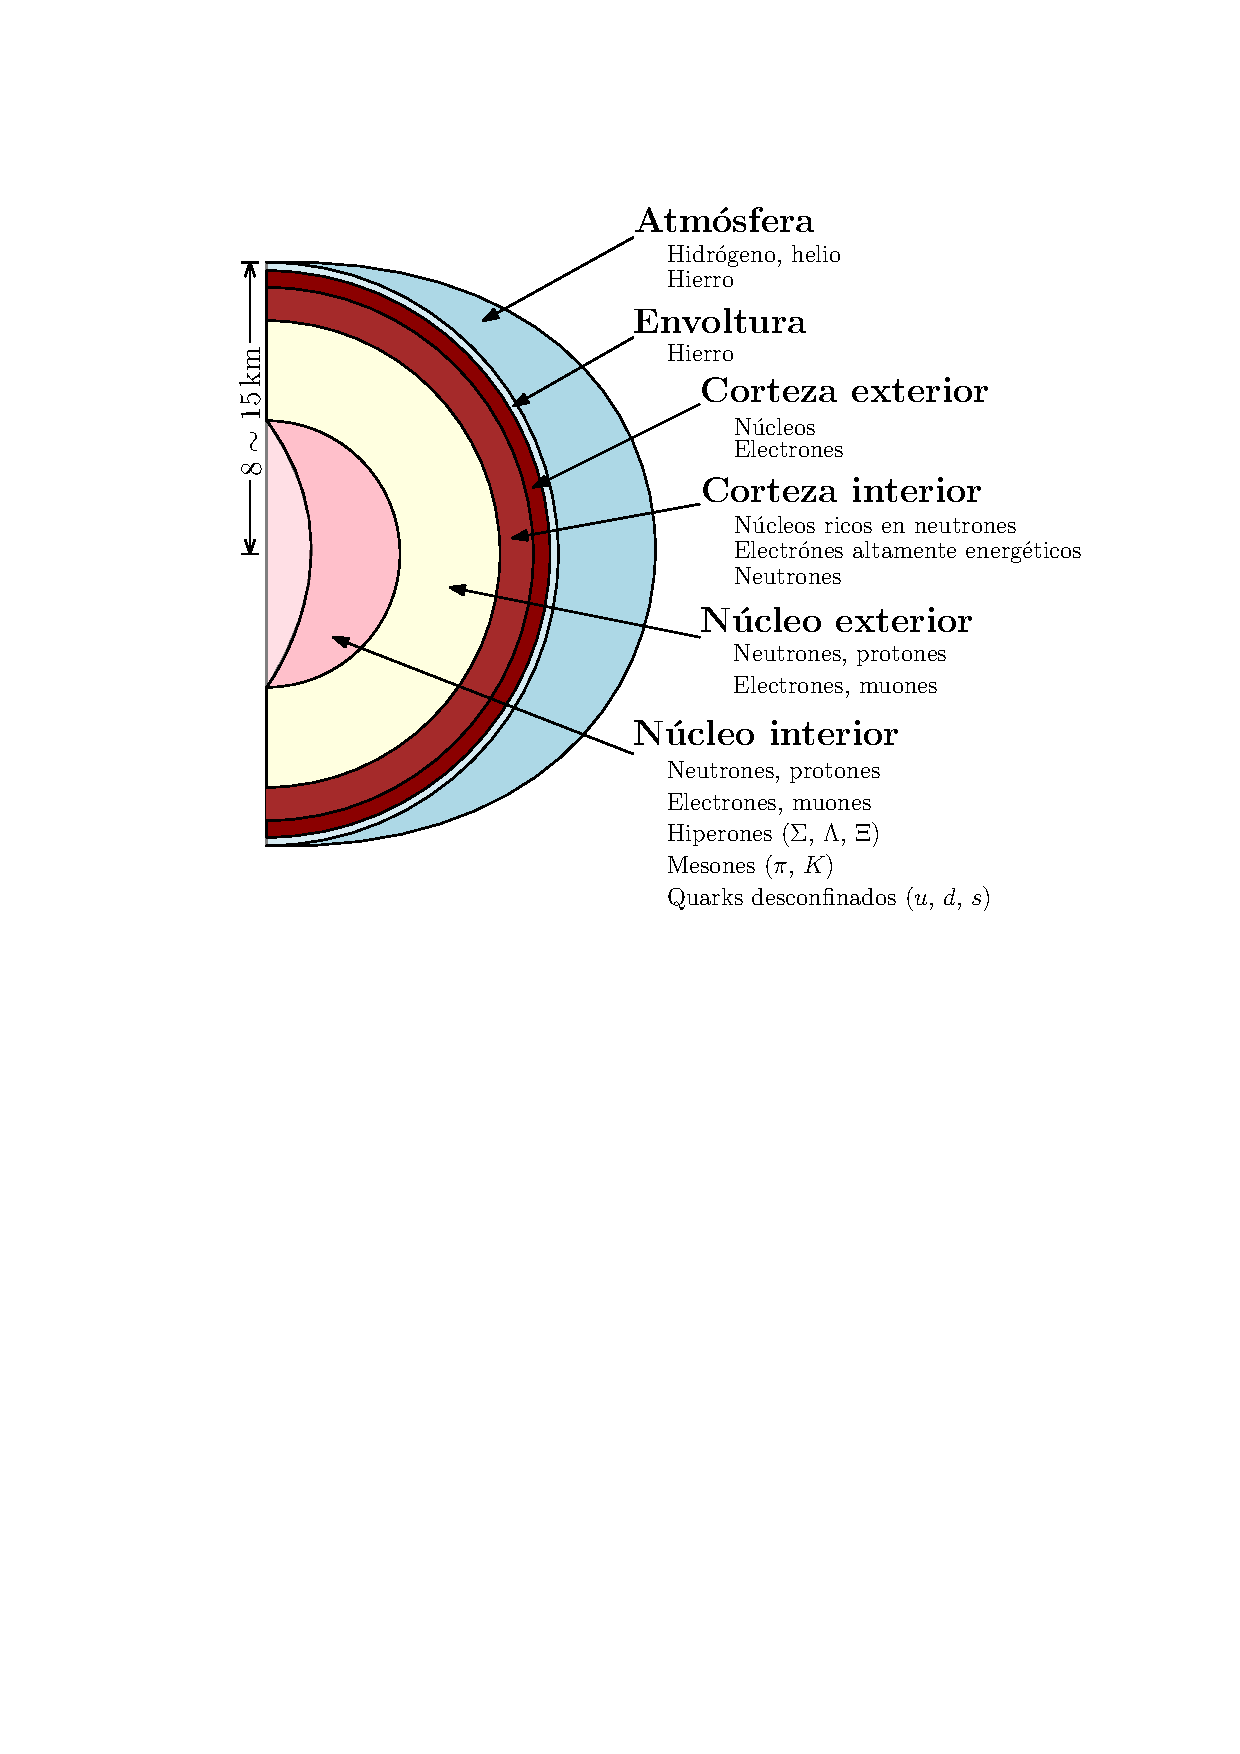
\includegraphics[width=300pt]{figures/neutronstar.pdf}
    \caption{Composición de una estrella de neutrones.\protect\footnotemark}
    \label{NSC}
\end{figure}
\footnotetext{Original: Figura 1 de \cite{Weber2012}}


El \emph{núcleo} comprende regiones en las que la densidad alcanza $\rho_0$ y contiene la mayor fracción de la masa estelar. Está subdividido un dos: el \emph{núcleo exterior}, con densidad $\num{0.5}\rho_0\lesssim\rho\lesssim 2\rho_0$  cuya composición se conoce bien cualitativamente \cite{Haensel2007NeutronStructure}: es un superfluido de neutrones y protones, con presencia de electrones y muones altamente degenerados. Del \emph{núcleo interior}, por el contrario, no se conoce su composición. Se ha sugerido la presencia de hiperones, piones, kaones e incluso quarks desconfinados (consultar las revisiones \cite{Potekhin,Lattimer2004} y referencias allí citadas).



La gran variedad de fases que se encuentran a medida de que la densidad aumenta en el interior de las estrellas de neutrones están ilustradas en la Figura \ref{NSS}. 

\begin{figure}[H]
    \centering
    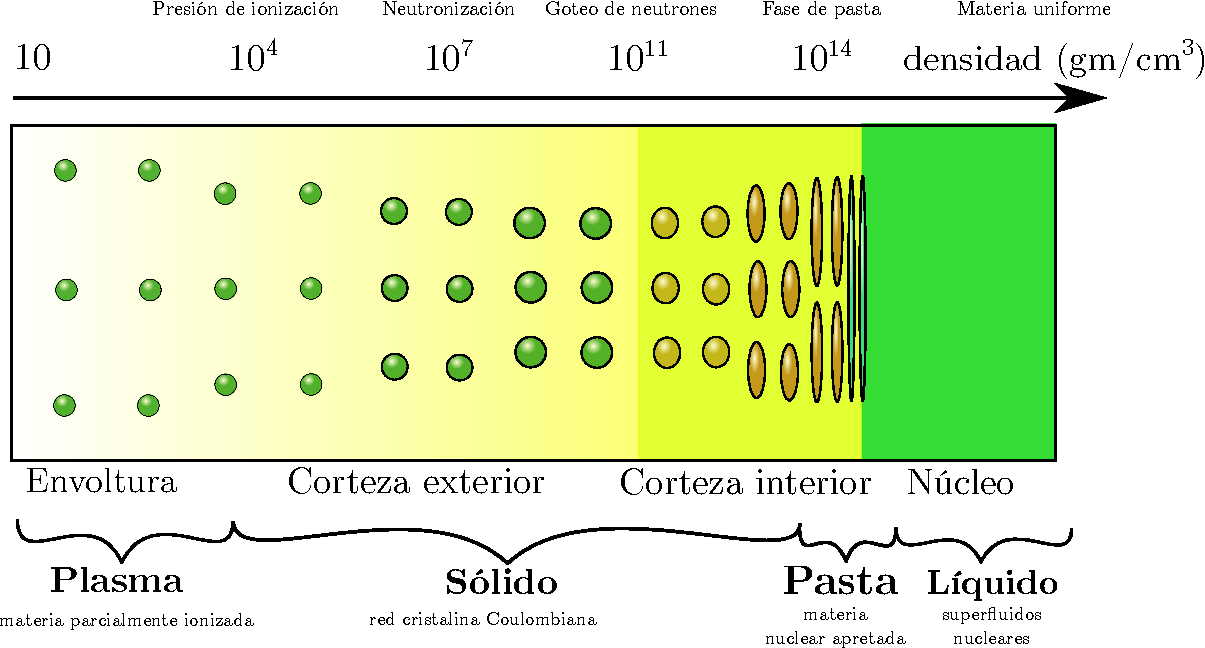
\includegraphics[width=420pt]{figures/Density.pdf}
    \caption[Estructura interna de una estrella de neutrones]{Estructura interna de una estrella de neutrones.\protect\footnotemark}
    \label{NSS}
\end{figure}
\footnotetext{Original: Figura 4 de \cite{Chamel2008}}   

\section{Ecuación de estado}

Como se mencionó en la Sección \ref{CR}, la ecuación de estado de la materia es necesaria para resolver las ecuaciones de TOV. Ésta se determina predominantemente de la interacción nuclear fuerte entre los constituyentes elementales de la materia y debido a que estas interacciones no son bien entendidas en materia a densidades superiores a la densidad de saturación nuclear $\rho_0$, la ecuación de estado de las estrellas de neutrones sigue siendo un misterio.

La mayoría de modelos de ecuaciones de estado se pueden agrupar en tres categorías: modelos de potencial no relativista, modelos de teoría de campos relativista y modelos de Dirac-Brueckner-Hartree-Fock relativistas. A continuación se presentarán algunos detalles de cada uno de estos enfoques.

\subsection{Modelos de potencial no relativista}
\subsection{Modelos de teoría de campos relativista}
\subsection{Modelos de Dirac-Brueckner-Hartree-Fock}